\documentclass{article}

\usepackage[letterpaper]{geometry}
\usepackage{graphicx}

\title{Multivarate Calculus Review}
\author{Duncan Wilkie}
\date{4 November 2021}

\begin{document}

\maketitle

\section{}
$f_x=-12xy$, $f_y=5y^4-6x^2$, and $f_{xy}=-12x$.

\section{}
\[(u,v)=(5,3)\]
\[\frac{\partial T}{\partial p}(1,2)=\left( \frac{\partial T}{\partial u}\frac{\partial u}{\partial p}+\frac{\partial T}{\partial v}\frac{\partial v}{\partial p}\right)(1,2)=\left( 3(p^2+q^2)^22p+3(p+q)^2 \right)(1,2)=177\]
\[\frac{\partial T}{\partial q}(1,2)=\left( \frac{\partial T}{\partial u}\frac{\partial u}{\partial q}+\frac{\partial T}{\partial v}\frac{\partial v}{\partial q} \right)(1,2)=\left( 3(p^2+q^2)^22q+3(p+q)^2 \right)(1,2)=327\]

\section{}
The first two can just be evaluated directly.
\[\lim_{(x,y)\to (1,1)}\frac{x^2+y^2}{x^2+2y^2}=\frac{2}{3}\]
\[\lim_{(x,y)\to(1,0)}\frac{x^2+y^2}{x^2+2y^2}=1\]
The last doesn't exist, as if one approaches zero along the path $y=0$ one obtains the limit 1 by L'Hopital, but if one approaches zero along the path $x=0$ one obtains the limit $\frac{1}{2}$ by the same reasoning.

\section{}
With the convention that $\theta$ is azimuthal,
\[x=\rho\sin\phi\cos\theta\]
\[y=\rho\sin\phi\sin\theta\]
\[z=\rho\cos\phi\]

\section{}
\[I=\int_0^2\frac{x^3}{3}+y\frac{x^2}{2}+\frac{x^2}{2}e^y\bigg|_0^1dy=\int_0^2\frac{1}{3}+\frac{y}{2}+\frac{e^y}{2}dy=\frac{y}{3}+\frac{y^2}{2}+\frac{e^y}{2}\bigg|_0^2=\frac{2}{3}+2+\frac{e^2}{2}-\frac{1}{2}\approx 5.8612\]

\section{}
The integrand is the volume element in spherical coordinates, so it is the volume of a cylinder of height 1.

\section{}
\[I=\int_0^2\int_{x^2}^{2x}xydydx=\int_0^2x\left( \frac{(2x)^2}{2}-\frac{x^4}{2}\right)dx=\frac{x^4}{2}\bigg|_0^2-\frac{x^6}{12}\bigg|_0^2=\frac{8}{3}\]

$\Omega$ is
\[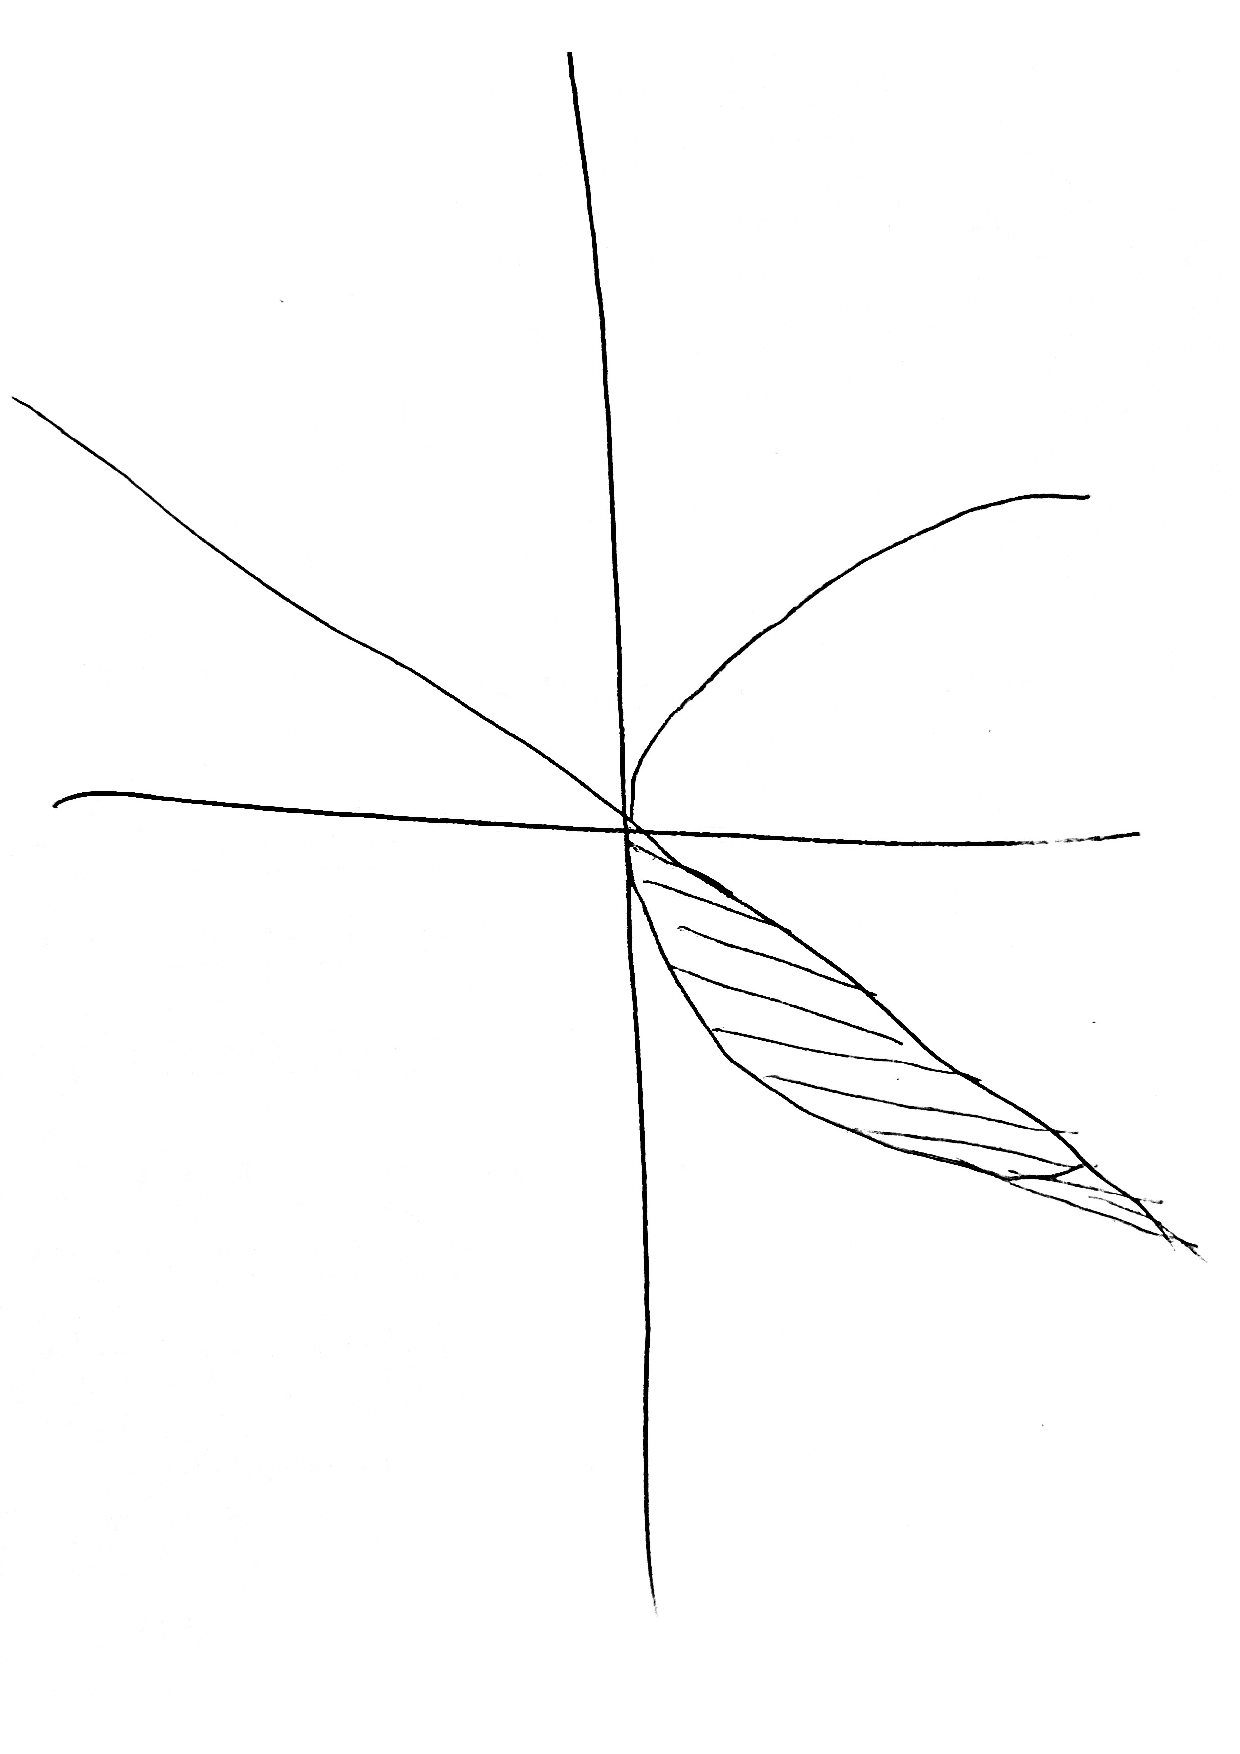
\includegraphics[scale=0.25, angle=90]{img.pdf}\]
\end{document}
%%% Local Variables:
%%% mode: latex
%%% TeX-master: t
%%% End:
